% !TeX root = ./main.tex

\section{Results}
\label{sec:results}
\subsection{Gridsearch \& Performance}
As mentioned in \ref{sec:training}, several scores were used to assess the quality of the models. After the grid search had finished, the best classifier configuration by the recall score was analyzed. As predicted, however, the best estimators chosen by the grid search algorithm, performed subpar in most of the other three tests. The chosen classifiers by the algorithm were then discarded and the results of the grid search were manually analyzed. The analysis was performed for each of the trained classifiers -- RFC, DTC, SVM. The five best configurations for every test were evaluated, but if one configuration performed worse than .6 in any score, it was not taken into consideration. Hence, a maximum of 20 configurations would be evaluated per model. But since often the best parameter combination led to top performance in all tests, there have not been 20 configurations for any model. There were nine decision tree classifiers, seven random forest classifiers and ten support vector machine classifiers left to analyze. The model performance for each of the tests was then plotted and the mean score over all scores calculated and compared (see figures \ref{fig:dtc_results}, \ref{fig:rfc_results}, \ref{fig:svm_results}). From this it was determined that DTC model 1, RFC model 7 and SVM model 447 were the best overall models. The grid search algorithm proposed DTC model 7 as the best classifier, but seeing that it performs well below the comparable models, model 1 was chosen instead. Model 1 also has the highest mean score. It achieved the highest average score of balanced accuracy and f1 and was still performing well in precision and recall. The grid search algorithm also proposed model 7 for the RFC selection, which turned out to work well and as such model 7 was retained as the best RFC configuration. Model 7 also has the highest mean score by 0.001. For the SVM configurations it proposed model 399. However, model 399 performed below .2 in precision and as such the f1 score was subpar as well and was hence excluded when selecting configurations for plotting. Its accuracy was a steady .5. However, most of the selected SVM configurations reach very similar top scores and most of the selected ten configurations would have been a reasonable choice. In the end, model 447 was chosen. While it does not have the highest mean score (that is on 555, and 447 ties with 540 and 342), 555 had a smaller recall and balanced accuracy score, and the high precision value skewed the mean. Hence the decision for 447.\\
\begin{figure}
    \centering
    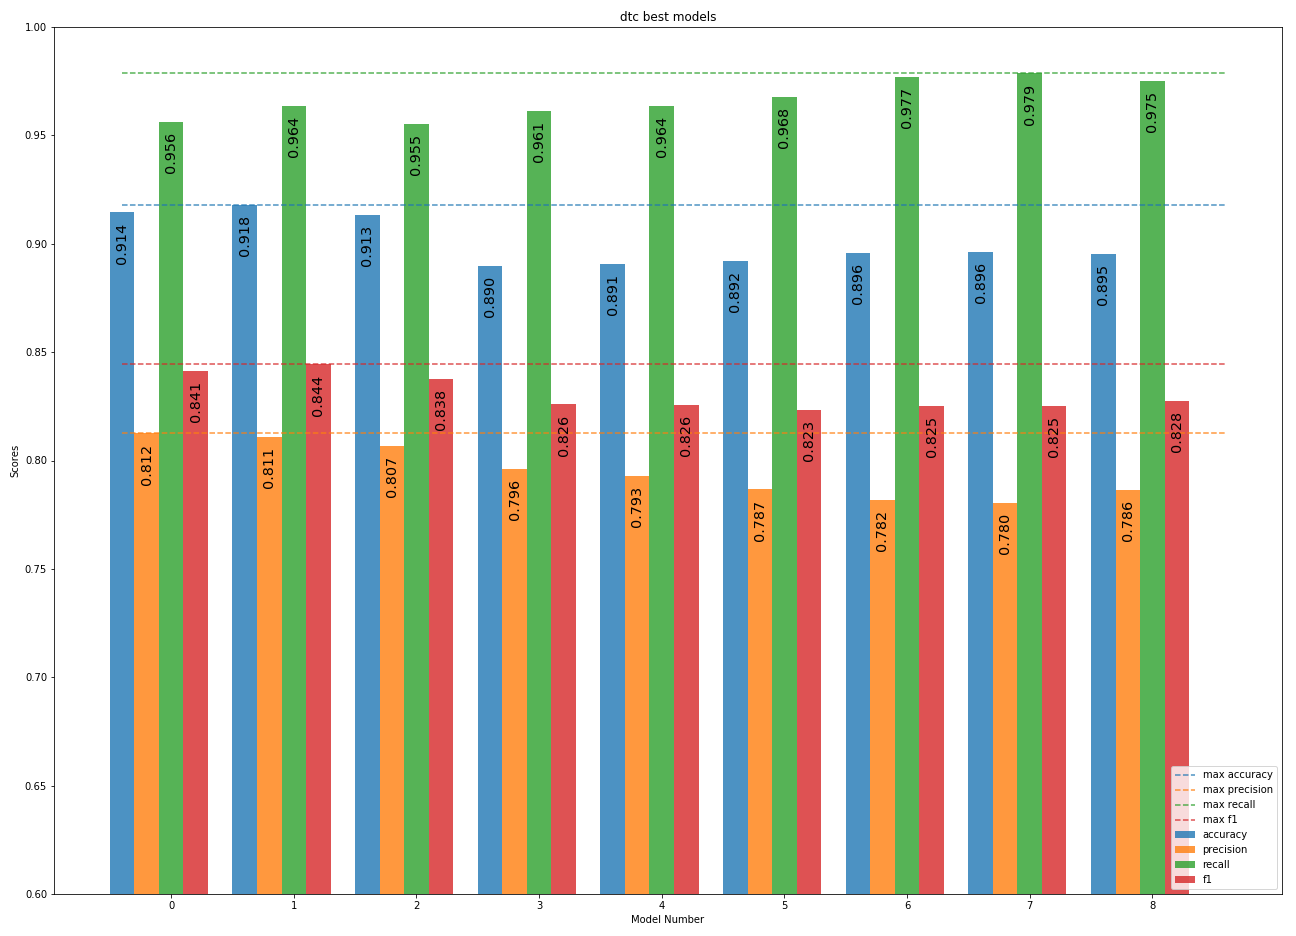
\includegraphics[width=.95\textwidth]{results_dtc.png}
    \mycaption{DTC results}{Performance of the best performing DTC configuration after the retraining}
    \label{fig:dtc_results}
\end{figure}
\begin{figure}
    \centering
    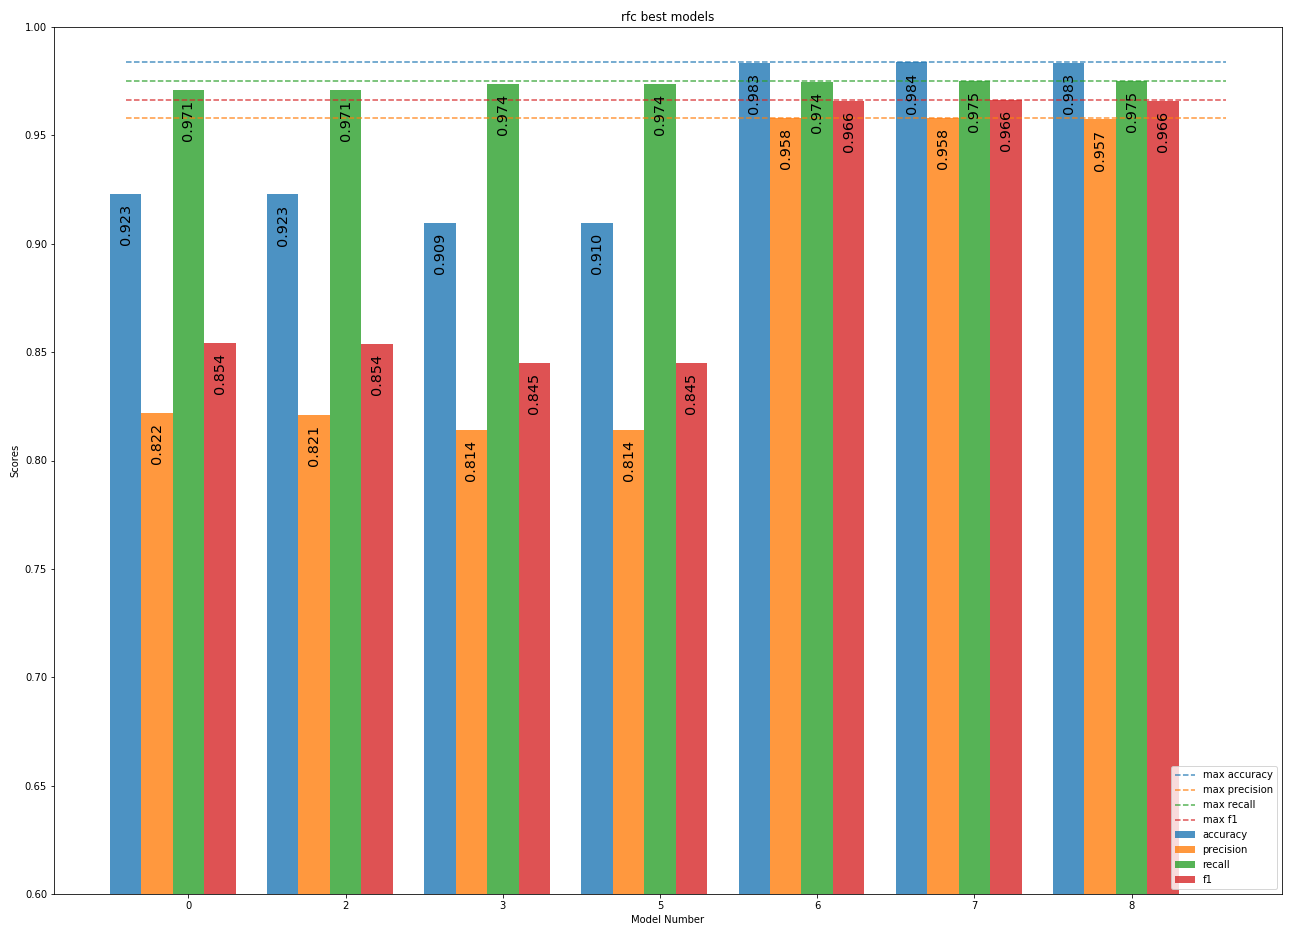
\includegraphics[width=.95\textwidth]{results_rfc.png}
    \mycaption{RFC results}{Performance of the best performing RFC configuration after the retraining}
    \label{fig:rfc_results}
\end{figure}
\begin{figure}
    \centering
    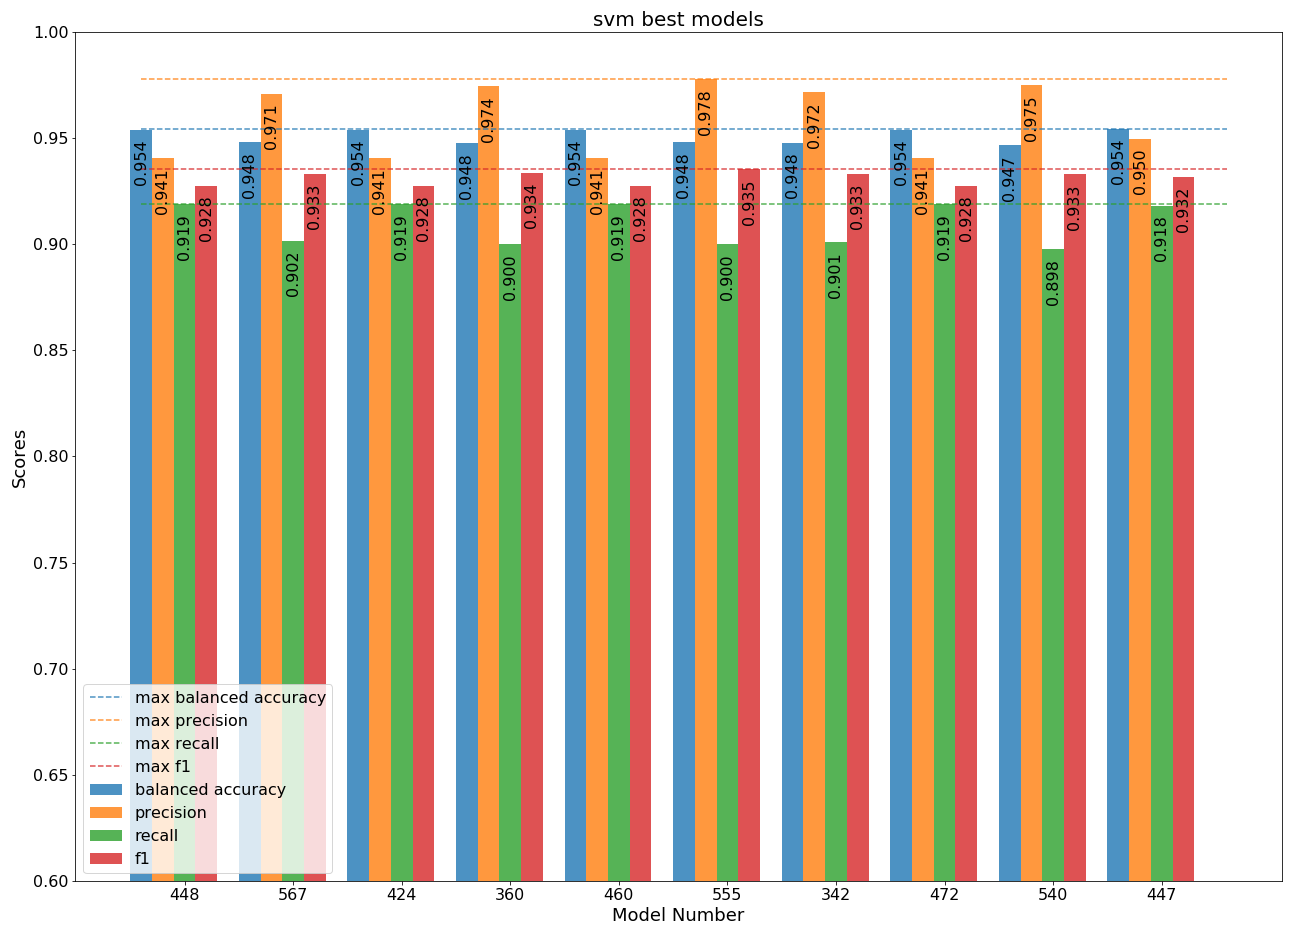
\includegraphics[width=.95\textwidth]{results_svm.png}
    \mycaption{SVM results}{Performance of the best performing SVM configuration after the retraining}
    \label{fig:svm_results}
\end{figure}
\FloatBarrier
The parameter configuration was then read out and a classifier was trained anew on the data to validate the grid search cross validation one last time. The resulting best performance configurations were:
\begin{description}
    \item [DTC:] Balanced class weight, gini impurity, 1 minimum sample per leaf, 3 minimum samples per split
    \item [RFC:] Balanced class weight, gini impurity, 5 minimum samples per leaf, 3 minimum samples per split
    \item [SVM:] Balanced class weight, polynomial kernel of degree 3, a gamma value of 0.00001, r=0, C = 100
\end{description}
In the end, all three ML algorithms performed well over expectations. They reached upper 90\% test scores in all employed scoring methods. Compared to the tree classifiers the support vector machine underperformed. This is probably due to the onehot encoding, leading to a blown up feature space and less information content in each dimension of that feature space. Given this altered dataset, the SVM still performed well. With a small edge the random forest classifier does perform the best out of all of them. This was to be expected, since the dataset consisted mostly of nominal data, and the random forest should always outperform the simple decision tree classifier.\\
The feed forward network on the other hand performed well below the other three. Deep learning architectures more often than not need a larger sample size to train and generalize well. But in many cases where such a dataset was available, deep learning did surpass other ML algorithms. In this case however, the dataset was comparably small, as discussed in \ref{sec:training}. Since the samples needed to be onehot encoded as well before fed into the FFN, the data had lost information and now contained more features than samples. A shallow, but wide architecture might have been able to perform decently on this task, but due to memory limitations of available hardware, this was not possible to evaluate. The configurations that were tried, had between one and five hidden layers, and between 128 and 2048 neurons in the first hidden layer; subsequent layers would get smaller until the readout layer with one single neuron was reached. The networks were tried with a sigmoidian and a ReLU activation function, whereas the readout layer was always using a sigmoidian function. None of these configurations performed above chance level (46\%-54\% mean accuracy). Since there was no sign of a well performing network, there were no resources spent on further automatic hyperparameter tuning. Following this, the FFN was left out on all evaluations.

\subsection{Feature Importances}
In order to get some insight into which variables were important when determining study success, the feature importances of the random forest classifier were analyzed. The feature importances of a random forest are the average importances over all trees as it is implemented in scikit learn. It was thus possible to calculate the standard deviation and average feature importance of all features. The svm has no interpretable weights. For the single decision tree, since there is only one feature ranking, there is no standard deviation. Looking at the feature importances, two things stand out. Firstly, there is a huge drop in feature importance after the very first feature and secondly, that first feature is a year variable, located in the vocational training spell file. During the preprocessing step of aggregating the spell files, the year variables were intentionally left out, to hold the classifiers more general. Since the vocational training file was handled as the basis to work on, it was not aggregated on its own and thus the year variables were not removed from the resulting frame. This would explain the excellent performance. A vocational spell ending in e.g. 2012, has a high probability of being an unsuccessful study episode, since the interviews started in 2010 and the majority of participants also took up their studies in 2010.\\
As a reaction to these results, all remaining year variables were removed and the classifiers retrained (Correction-1). There were no resources to employ a full grid search again, but since the dataset changed only slightly, the best classifier configurations from above were used again. Removing the year variable lead to a decrease in performance. This was to be expected, judging by the large discrepancy between the importance of the year variable and all other features. After training and testing was done, the feature importances were read out and analyzed again. Two variables stuck out, again leading by a large margin. Upon further inspection, those variables turned out to be "Grade Vocational qualification" (ts15265) and "Vocational qualification" (ts15219\_v1). ts15265 has a value for 6309 successful studies (that is 97.75\% of that class), but only for 954 unsuccessful studies (30.80\% of class). Similarly, ts15219\_v1 has a value for 5808 successful spells, but only 1029 unsuccessful spells. Again there were variables which were allowing the algorithms to "cheat". ts15265 as well as ts15219\_v1 are clear indicators whether a spell was completed successfully. The algorithm will not have to learn the patterns of the data, but rather just to learn the correlation of these two variables and the target value.\\
The two variables were removed from the dataset as well, and the classifier retrained and analyzed again (Correction-2). The drop off from the first feature to the following ones has grown considerably. The now most important feature is "Vocational training with at least 1 month aborad completed" (ts15223). Less important were the average net income during employmet and "successful in studies compared to others". ts15223 does not indicate an already completed spell. Time spent abroad for the vocational education might indicate a higher semester and with this a higher chance of successful completion.\\
Additionally, a joined dataframe without any information from VocTrain was created, since there seemed to be an unknown amount of variables strongly indicating a successful study spell. Due to resource limitations again no grid search was employed, but the model configuration identified in the first steps were retrained on this dataset (Without VocTrain). Without VocTrain, the dataset was shrunk to $9551 \times 848$ and $9551 \times 13912$ onehot encoded. Since the resulting dataset had no collected information on the vocational spell, the data was instead sampled from CATI and CAWI. The most important features changed, but are still related to the data found in VocTrain (see figure \ref{fig:no_voctrain_feature_importances}).\\
For an overview of the variables of feature importance see table \ref{tab:feature_importances}.

There is an interesting change from Correction-2 to Without VocTrain. Firstly, the standard deviation increased drastically, implying more unstable predicitive features. tg51300\_v1 appears to be used by many trees of the RFC, but there is also a good number of trees not using this variable as an important feature. Additionally, the classifier resorted to picking variables from CAWI and CATI related to vocational education.
\begin{figure}
    \centering
    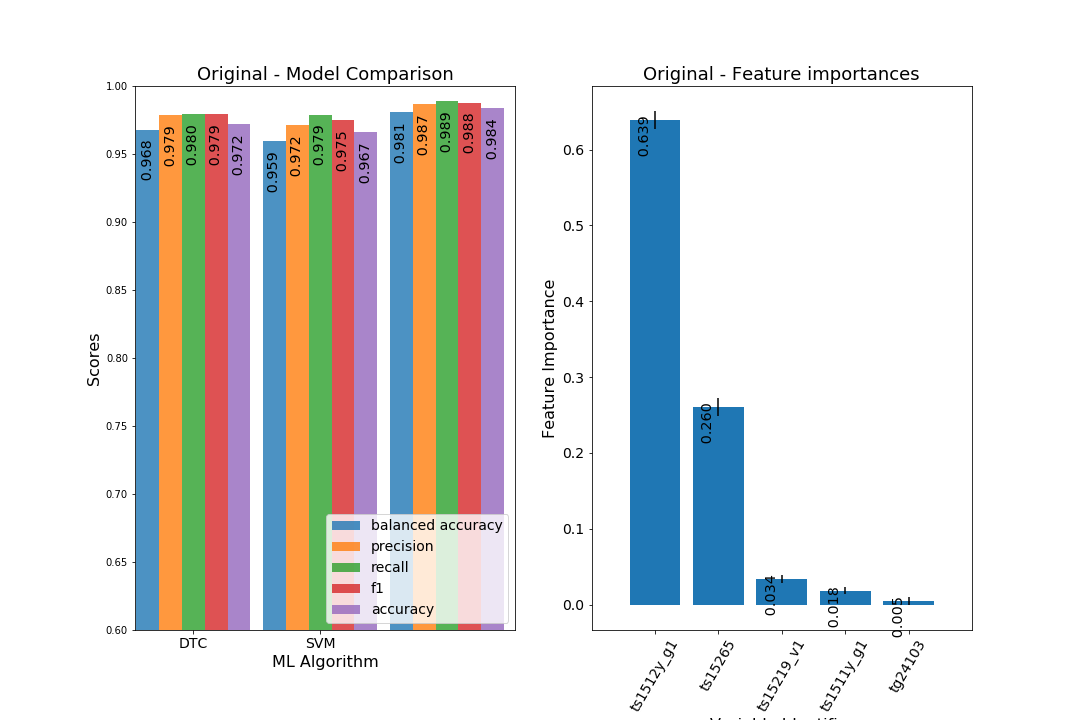
\includegraphics[height=.35\textheight]{eval_Original}
    \mycaption{Feature Importances, Original Run}{Feature importances of the RFC after the first run}
    \label{fig:old_feature_importances}
\end{figure}
\begin{figure}
    \centering
    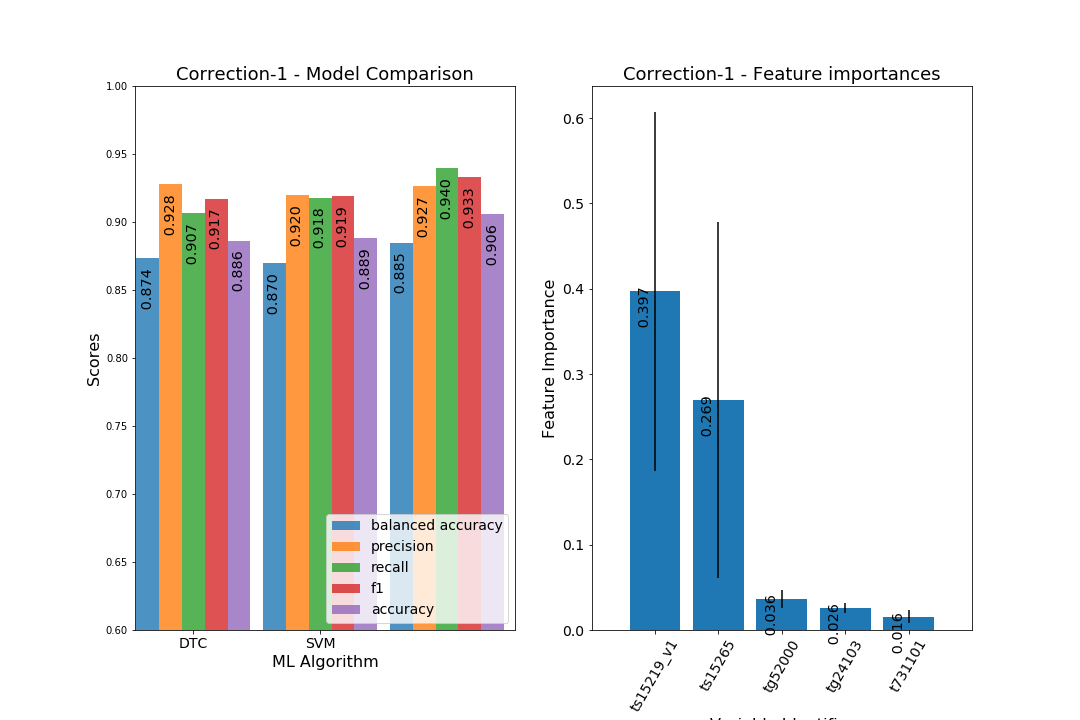
\includegraphics[height=.35\textheight]{eval_Correction-1}
    \mycaption{Feature Importances, Correction 1}{Feature importances of the RFC after removing the missed year variables}
    \label{fig:int_feature_importances}
\end{figure}
\begin{figure}
    \centering
    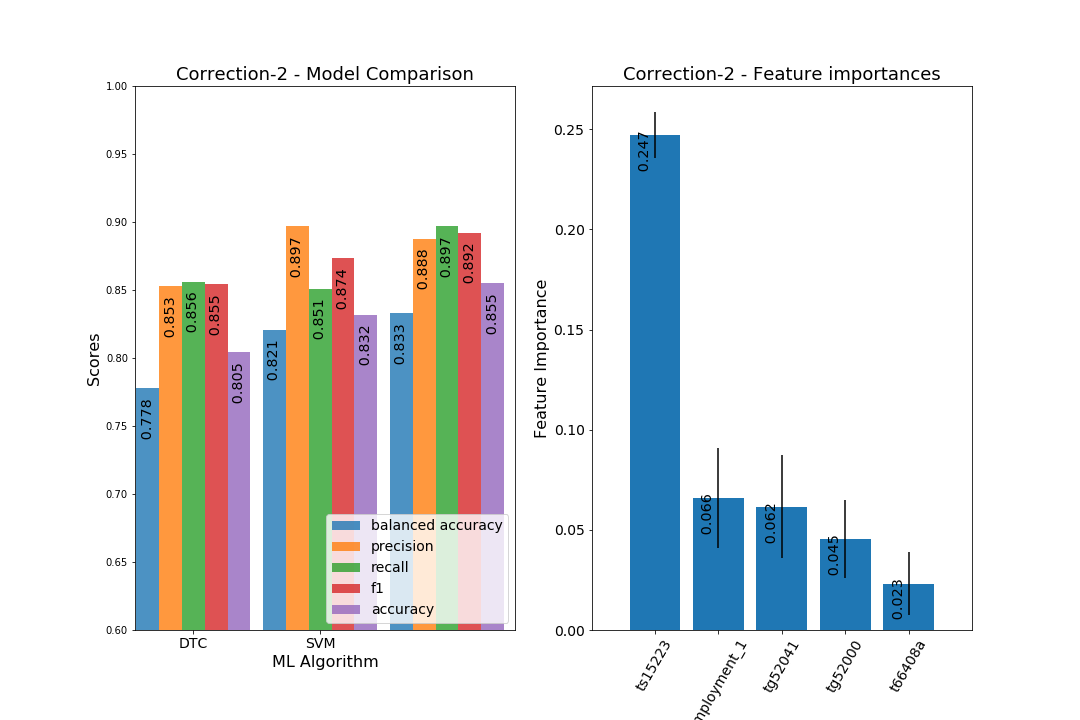
\includegraphics[height=.35\textheight]{eval_Correction-2}
    \mycaption{Feature Importances, Correction 2}{Feature importances of the RFC after removing the auxillary variable, holding the highest degree obtained}
    \label{fig:newer_feature_importances}
\end{figure}
\begin{figure}
    \centering
    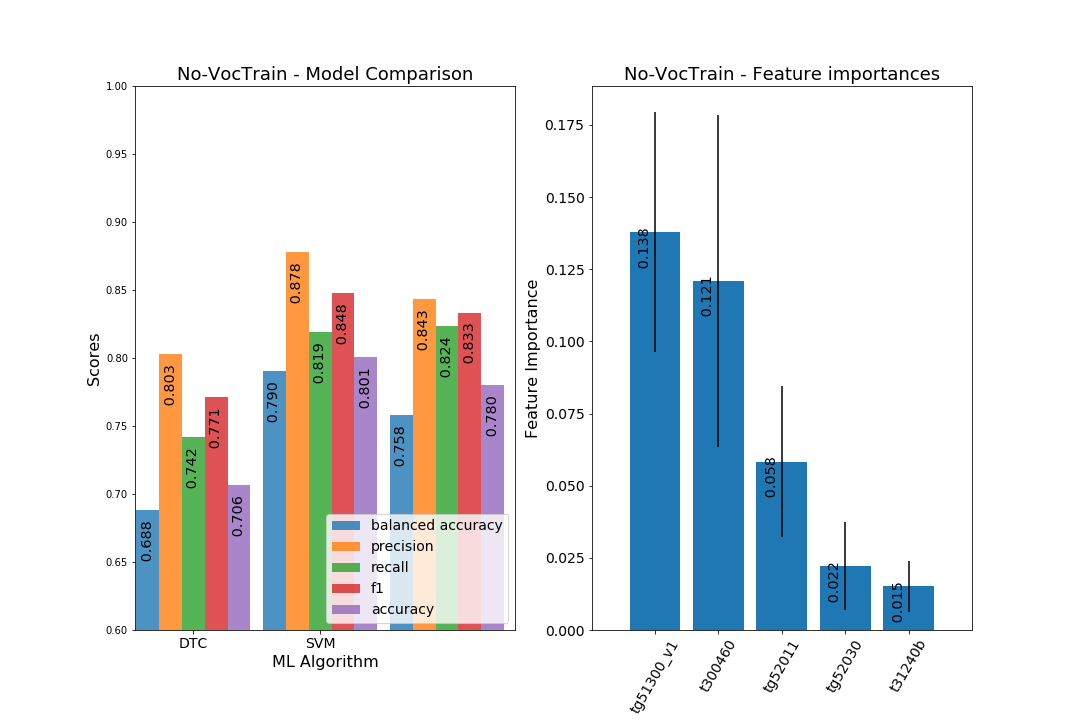
\includegraphics[height=.4\textheight]{eval_No-VocTrain.png}
    \mycaption{Feature Importances, Without VocTrain}{Feature importances after removing the VocTrain file completley from the dataset}
    \label{fig:no_voctrain_feature_importances}
\end{figure}
\begin{table}
    \centering
    \mycaption{Feature Importances: Variablenames}{The corresponding variable names for the features extraced, sorted by run}
    \label{tab:feature_importances}
    \begin{tabular}{p{.25\textwidth} p{.65\textwidth}}
        \textbf{Variable} & \textbf{Variable Name}\\
        \hline
        \multicolumn{2}{c}{Without VocTrain}\\
        \hline
        tg51300\_v1  & 	 Field of study changed since last survey\\
        t300460 & 	 Subjective probability of obtaining a Master’s degree\\
        tg52011 & 	 ECTS points achieved so far\\
        tg52030 & 	 Correspondence study workload with study regulations?\\
        t31240b & 	 Change of major subject\\
        \hline
        \multicolumn{2}{c}{Correction-2}\\
        \hline
        ts15223 & 	 Vocational training with at least 1 month abroad completed\\
        employment\_average\_net\_income & 	 employment\_average\_net\_income\\
        tg52041 & 	 successful in studies compared to others\\
        tg52000 & 	 Performance evaluation according to ECTS?\\
        t66408a & 	 Motivation: Future career opportunities\\
        \hline
        \multicolumn{2}{c}{Correction-1}\\
        \hline
        ts15219\_v1 &	 Vocational qualificaon\\
        ts15265 &	 Grade Vocational qualification\\
        tg52000 &	 Performance evaluation according to ECTS?\\
        tg24103 &	 Episode mode\\
        t731101 &	 Family structures up to age 14\\
        \hline
        \multicolumn{2}{c}{Original}\\
        \hline
        ts1512y\_g1  &   Biography: Ending date of spell (year, edited)\\
        ts15265 &   Grade Vocational qualification\\
        ts15219\_v1  &   Vocational qualification\\
        ts1511y\_g1  &   Biography: Starting date of spell (year, edited)\\
        tg24103 &   Episode mode\\
    \end{tabular}
    % No-VocTrain
    % tg51300_v1 	 Fachwechsel seit letzter Befragung
    % t300460 	 Subjektive Erfolgswahrscheinlichkeit  Studienabschluss Master
    % tg52011 	 bislang erreichte ECTS-Punkte
    % tg52030 	 Entsprechung Studienpensum mit Studienordnung?
    % t31240b 	 Studienwechsel
    
    % Original
    % ts1512y_g1 	 Prüfmodul: Enddatum (Jahr, ediert)
    % ts15265 	 Note Ausbildungsabschluss
    % ts15219_v1 	 Ausbildungsabschluss
    % ts1511y_g1 	 Prüfmodul: Startdatum (Jahr, ediert)
    % tg24103 	 Episodenmodus
    
    % Correction-1
    % ts15219_v1 	 Ausbildungsabschluss
    % ts15265 	 Note Ausbildungsabschluss
    % tg52000 	 Leistungsbewertung nach ECTS?
    % tg24103 	 Episodenmodus
    % t731101 	 Familienform bis zum 15. Lebensjahr
    
    % Correction-2
    % ts15223 	 Ausbildung mind. 1 Monat im Ausland absolviert
    % tg51116 	 akt. Tätigkeit: Vikariat
    % tg52000 	 Leistungsbewertung nach ECTS?
    % employment_average_net_income 	 employment_average_net_income
    % tg24103 	 Episodenmodus
    
    % Correction-3
    % ts15223 	 Ausbildung mind. 1 Monat im Ausland absolviert
    % employment_average_net_income 	 employment_average_net_income
    % tg52041 	 erfolgreich im Studium verglichen mit anderen
    % tg52000 	 Leistungsbewertung nach ECTS?
    % t66408a 	 Motivation: spätere Berufschancen
\end{table}